%%%% PLEASE REPLACE ENTIRELY WITH YOUR OWN CONTENT %%%%


\chapter{Metodologia / desenvolupament del projecte}
  
  En aquest capítol es detallarà la metodologia emprada en la realització del treball. Té com a objectiu oferir un compte detallat de les aproximacions i tècniques utilitzades, assegurant la replicabilitat i el rigor acadèmic. No només cobrirà els mètodes de recerca i tècniques de mesurament emprats, sinó que també aprofundirà en les especificitats del desenvolupament de programari i maquinari. Tant si el projecte implica anàlisi qualitativa, mesuraments quantitatius, modelatge computacional com prototipatge físic, aquest capítol hauria d'elucidar com contribueix cada component als objectius generals.
  
  A més de descriure els mètodes en si mateixos, el capítol també proporcionarà justificacions per què es van escollir mètodes particulars enfront d'altres. Per exemple, podria explicar la tria d'un llenguatge de programació específic, prova estadística o configuració experimental. El capítol també abordarà les limitacions de la metodologia i com aquestes s'han mitigat o tingut en compte. Els lectors haurien de sortir amb una comprensió clara de com s'ha dut a terme el desenvolupament del projecte, per què s'han escollit determinades opcions i com aquests mètodes serveixen per complir els objectius establerts inicialment.

\section{Escenari utilitzat}

  L’escenari presentat en aquest treball està inspirat en el que s'utilitza en el Treball: \textit{" «MIoTTA-UPC: Testbed MIoT Configurable para la Evaluacion de Algoritmos de Detección de Ciberataques Basados en Inteligencia Artificial» "} \cite{miottaupcfig} . L’objectiu principal és poder generar un banc de dades que contingui paquets benignes i maliciosos de diferents atcas per a entrenar un sistema de detecció d’intrusions (IDS) basat en intel·ligència artificial que classifiqui si aquest tràfic és benigne o maliciós. La programació, desplegament i entrenament d’aquest IDS no formen part d’aquest treball. Per a generar aquest testbed és necessari simular atacs coneguts per a una infraestructura com utilitzada de manera realista i amb un escenari que reprodueixi adequadament unes condicions reals.

\section{Topologia general}
\label{sec:Topologia}
  Per a la generació i captura del tràfic de xarxa en un IoMT (Internet of Medical Things), s’ha dissenyat i desplegat un escenari experimental que simula una habitació d’hospital interconnectada amb un servidor central i altres dispositius de suport clínic. Aquest entorn busca reproduir amb fidelitat un ecosistema típic d’atenció sanitària digitalitzada, incloent-hi sensors mèdics, passarel·les de comunicació, equips de monitoratge i possibles actors maliciosos.


  L’escenari està basat en una xarxa LAN Wi-Fi irradiada amb un Access Point, en la qual s’hi connecten tots els dispositius, encara que també pot contenir trams Ethernet si és necessari. Entre els dispositius utilitzats es considera:

  \begin{itemize}
    \item \textbf{Clients MQTT:} Aquests clients són sensors com ara oxímetres, monitors de ritme cardíac, bombes d’infusió, sensors de glucosa, tensiòmetres o altres sensors utilitzats en l’entorn mèdic. Aquests clients poden actuar tant transmetent informació a altres dispositius com esperant rebre’n o ambdues a la vegada. Una part d’aquests dispositius, s’implementarà de forma simulada i injectada a la xarxa a través d’un node comú, ja que es tracta de dispositius amb gran cost econòmic. En aquest treball s’utilitzarà Docker com és explicat en apartats posteriors.
    \item \textbf{Broker MQTT:} Connectat a la xarxa, es disposa d’un servidor o broker MQTT amb el el qual s’hi connecten sigui per enviar o rebre informació tots els clients de la xarxa. Actua com un organisme central de la informació i un punt crític de la xarxa.
    \item \textbf{Atacant:} Dintre aquesta xarxa Wi-Fi, se suposa que es connecta un dispositiu atacant, el qual realitza diversos atacs cap als altres components de la xarxa.
    \item \textbf{Monitor de trànsit:} S’hi connecta un monitor que captura tot el trànsit dins la xarxa visible des de la seva posició. Aquest actua de forma passiva escoltant tot el trànsit que circula i recopilant tota la informació possible per tal generar el \textit{testbed}, que és el principal objectiu del treball.
    \item \textbf{Ordinadors I servidors:} Se suposa que en aquesta xarxa hi poden haver connectats altres dispositius que no són especialment utilitzats en l’entorn IoMT com per exemple altres servidors hospitalaris o ordinadors.
  \end{itemize}

  Dintre aquest escenari, el meu treball se centra en l’apartat de la generació de trànsit simulat així com en l’elaboració d’atacs des de la perspectiva de desplegar clients simulats i fer-los interactuar amb la xarxa real. L’objectiu principal del treball no ha estat la implementació d’aquesta xarxa.

  \begin{figure}[H]
    \centering
    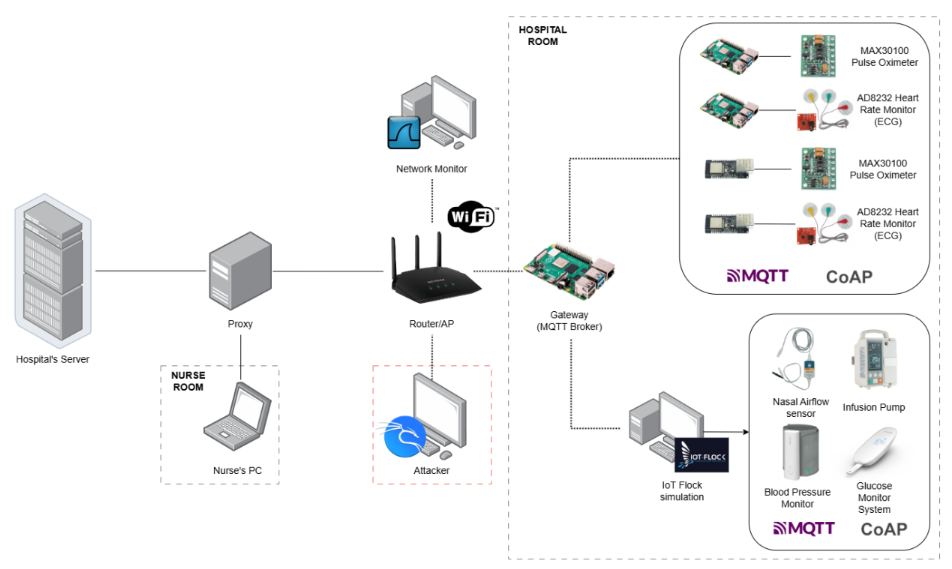
\includegraphics[width=1\textwidth]{img/MIOTTA_UPC.png}
    \caption{Esquema de l'arquitectura utilitzada. Imatge extreta del treball \cite{miottaupcfig}.}
    \label{fig:MQTT}
  \end{figure}

\section{Ús del protocol MQTT}
  Primer de tot, l’elecció del protocol MQTT (Message Queuing Telemetry Transport) està fonamentada en el fet que és un dels protocols més utilitzats en l’àmbit IoT en general i en entorns IoMT en específic.

  És un dels protocols amb més rellevància i eficiència per a dispositius amb recursos limitats, com és el cas d’aquest treball, on l’apartat de les comunicacions no és la seva funció principal. Consta d’una arquitectura \textit{publisher – subscriber} centralitzada en un únic servidor, la qual cosa fa que tota la informació estigui centralitzada en un sol dispositiu, aquest fet el fa vulnerable i, per tant, cal prendre les mesures de seguretat adequades. A més a més, és un protocol altament configurable, ja que s’hi poden configurar mesures de seguretat com ara limitacions de trànsit, Access Lists (ACL) o encriptat TLS.

  Dintre aquest projecte del grup ISG-UPC també es contempla el protocol CoAP, més enfocat a una arquitectura client -servidor semblant a protocols HTTP, però en aquest treball no serà utilitzat.

  \label{sec:mosquitto}
  Mosquitto és una de les implementacions més conegudes del protocol MQTT. Es tracta d’un broker MQTT lleuger, de codi obert i altament configurable i compatible amb les especificacions MQTT 3.1 i 5.0 que permet la configuració de les funcionalitats bàsiques del protocol com definir tòpics, limitacions en l'ús de recursos, ACLs I encriptat TLS. També permet desplegar clients MQTT mitjançant mosquitto-clients i poder realitzar el procés de subscriure’s a un tòpic en un broker concret (mosquitto-sub) on publicar missatges en aquest tòpic (mosquitto-pub). Adicionalment, disposa de les configuracions bàsiques de MQTT com els paràmetres de QoS, retain o presistance. \cite{Mosquittoexp}

  En l’entorn acadèmic, la seva simplicitat fa que sigui una excel·lent opció per a desplegar laboratoris d’IoMT.
  \label{sec:Paho-MQTT}
  També és important destacar la llibreria Paho-MQTT que permet implelentar clients MQTT a través de Pytthon i és molt útil per a tasques d'automatització i scripting en entorns IoT. 


\section{Ús de Docker per al desplegament de dispositius}
\label{sec:Docker}
  Per al desplegament dels dispositius simulats (clients) i del servidor MQTT (broker), s’ha optat per l’ús de contenidors Docker en lloc de màquines virtuals (VMs). Aquesta decisió s’ha pres tenint en compte diversos criteris tècnics, pràctics i de rendiment, que fan que Docker sigui una opció més adequada per als objectius del projecte.

  Docker et permet desplegar contenidors seguint una imatge comuna i configurable. D’aquesta manera, podem desplegar els clients simulats o el servidor en qualsevol entorn i sistema que compleixi uns requisits mínims de hardware I software. També permet mantenir una eficiència de recursos òptima, ja que utilitza el propi kernel del sistema hipervisor.

  Alhora, és un sistema aïllat del sistema operatiu principal, per això, podem executar proves de penetració sense veure compromesa realment la seguretat dels nostres equips i amb una gran facilitat de reproduir aquest atac diverses vegades sense haver de configurar novament tot el dispositiu vulnerat, ja que aquests contenidors són fàcilment renovables per còpies idèntiques prèvies a l'atac.
  
  A través del seu orquestrador Docker Compose, podem realitzar desplegaments múltiples de dispositius. Amb aquesta eina, podem desplegar en un sol dispositiu físic una gran quantitat de dispositius simulats que comparteixin unes característiques comunes entre ells.

  Dintre dels motius pels quals s’ha escollit aquesta tecnologia, està l’ús de volums, els quals et permeten compartir espai en memòria entre el dispositiu hipervisor i els contenidors. Aquesta funcionalitat ens permet agilitzar la transferència d’arxius entre contenidors, com ara fitxers de configuració, scripts per executar tasques determinades o atacs coordinats (en el cas de contenidors desplegats per l’atacant).

  També he utilitzat l’arquitectura de xarxa de Docker Compose per a poder crear infraestructures de xarxa simulades senceres, mantenint una lògica i rigorositat en les adreces de cada contenidor, d’aquesta manera, per a alguns atacs m’és possible simular una arquitectura com ara una gran quantitat de contenidors connectats a un switch o bé com un seguit de serveis del host per fer una arquitectura de microserveis dintre un mateix dispositiu.

  \begin{figure}[H]
    \centering
    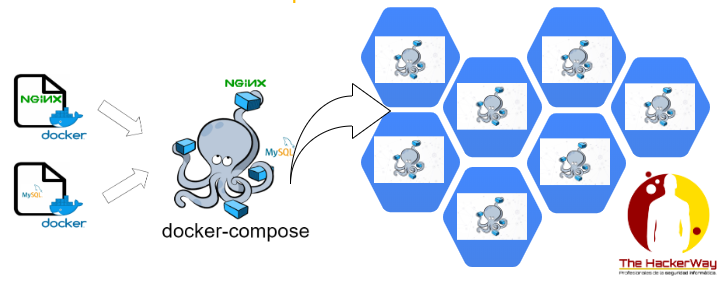
\includegraphics[width=1\textwidth]{img/DockerFig.png}
    \caption{Esquema de la generació de contenidors amb Docker Compose. Imatge extreta de \textit{The Hacker Way} \cite{miottaupcfig}.}
    \label{fig:MQTT2}
  \end{figure}




\section{Eines utilitzades per a la generació d'atacs}
\label{sec:Eines}
  Per a la realització d’aquest treball s’han emprat diverses eines de codi obert, escollides pel seu suport ampliat en entorns de xarxa, la seva flexibilitat i la possibilitat d’automatitzar proves i captures de trànsit en entorns simulats. Algunes d’aquestes eines tenen un enfocament general i són àmpliament utilitzades en proves de penetració en xarxes IP tradicionals, mentre que d’altres presenten característiques específiques que les fan especialment adequades per a entorns IoT o IoMT.

  Totes aquestes eines han estat utilitzades en un entorn de Kali Linux, que és l’entorn base per a la realització d’aquest treball. 
  
  Kali Linux és una distribució basada en Debian orientada específicament a seguretat informàtica i proves de penetració (pentesting). Mantinguda per l’equip d’Offensive Security (OFSEC), Kali proporciona un entorn completament equipat amb centenars d’eines preinstal·lades per a l’auditoria de xarxes, anàlisi de vulnerabilitats, enginyeria inversa, sniffing, spoofing, explotació i forense digital. \cite{kaliexp} 
  
  Aquesta distribució té certes avantatges respecte a altres sistemes operatius, les mes destacables són:
    
    \begin{itemize}
      \item \textbf{Gran nombre d’eines incloses:} Kali inclou eines com Nmap, Masscan, Wireshark, tcpdump, Scapy, aprscan i moltes més, facilitant la realització de proves diverses sense necessitat d’instal·lació addicional.
      \item \textbf{Entorn controlat i configurable:} Kali pot executar-se de manera virtualitzada (en aquest treball s'ha utilitzat en contenidors Docker), fet que permet recrear escenaris controlats i aïllats per a la simulació d’atacs sense posar en risc cap sistema real.
      \item \textbf{Actualitzacions contínues i suport actiu de la comunitat:} Es tracta d’una distribució mantinguda amb freqüència, compatible amb la majoria d’arquitectures, i àmpliament utilitzada tant en àmbits acadèmics com professionals.
      \item \textbf{Automatització i scripting:} El seu entorn Unix-like facilita l’ús d’scripts en bash o python per automatitzar atacs, recollir trànsit o llançar seqüències repetitives d’accions
    \end{itemize}  

    A continuació es descriuen les principals fetes servir en aquest projecte:

    \subsection{Nmap}
    \label{sec:NMAP}
    Nmap (Network Mapper) és una eina de network reconnaissance i auditoria de xarxes molt utilitzada en l’àmbit del pentesting. Permet identificar dispositius connectats a una xarxa, descobrir serveis oberts, detectar sistemes operatius i obtenir informació detallada mitjançant scripts del motor NSE (Nmap Scripting Engine). Nmap pot utilitzar diferents tècniques d'escaneig (TCP SYN, UDP, ping sweep, etc.), i també permet la detecció de versions de serveis, cosa que facilita la identificació de vulnerabilitats específiques en dispositius o serveis actius. És una eina molt completa per a la fase de reconeixement, però pot resultar relativament lenta quan s’aplica a xarxes amb un gran nombre d’hosts o rangs amplis d’adreces IP.

    Masscan, en canvi, és una eina especialitzada en escaneig de ports oberts a gran escala i amb una velocitat molt superior a la de Nmap. La seva arquitectura li permet enviar milions de paquets per segon, fet que la fa ideal per a fer un descobriment ràpid d’hosts actius en xarxes grans. No proporciona tants detalls com Nmap (com versions de serveis o sistema operatiu), però és extremadament útil com a pas previ per detectar ràpidament quins dispositius responen en determinats ports.

    En el context d’aquest treball, Masscan ha resultat especialment útil per a detectar dispositius IoT actius dins segments de xarxa amb centenars d’IPs possibles, abans d’aplicar anàlisis més profundes amb Nmap. Així, s’ha pogut optimitzar el temps d’escaneig i enfocar els esforços de reconeixement detallat només sobre aquells nodes que realment presentaven algun servei obert.

    \subsection{TCPDump}
    \label{sec:TCPDump}
    TCPDump és una eina de línia de comandes per a la captura i anàlisi de paquets a nivell de xarxa. Es tracta d’una eina fonamental en entorns de recerca i pentesting, ja que permet registrar amb precisió tot el trànsit que circula per una interfície de xarxa en temps real. \cite{wtfexp}
    
    TCPDump permet capturar trànsit benigne i maliciós entre dispositius de la xarxa i crear arxius de captura amb extensió pcap. És una eina similar a Wireshark, però més lleugera, utilitzada a través de terminal i amb capacitat de ser feta servir en automatitzacions.

    \subsection{ArpSpoof i Bettercap}
    \label{sec:ARPSpoof}
    ARPSpoof és una eina clàssica inclosa dins la suite dsniff, utilitzada per dur a terme atacs de tipus ARP spoofing o ARP poisoning. Aquest tipus d’atac consisteix a enviar respostes ARP falses dins una xarxa local per tal d’enganyar els dispositius i fer-los creure que l’atacant és el un altre dispositiu de la xarxa. Això permet interceptar el trànsit entre dos nodes, amb la finalitat de capturar dades sensibles o manipular el contingut dels paquets. ARPSpoof és una eina senzilla i directa, útil per entendre els fonaments d’aquest tipus d’atacs.

    BetterCAP, per la seva banda, és una eina molt més avançada i modular, dins d'ella s'inclouen funcionalitats per a realitzar atacs de tipus ARP spoofing més elaborats i personalitzables que amb ArpSpoof.

    \subsection{Mitmproxy}
    \label{sec:MITMProxy}
    MITMProxy és una eina de tipus proxy intermediari que permet interceptar, analitzar, modificar i registrar el trànsit entre clients i servidors de manera interactiva. A diferència d'altres eines centrades únicament en la captura passiva, MITMProxy ofereix una interfície potent per veure i modificar les peticions i respostes en temps real.

    Per a la realització d'aquest treball MITMProxy ha estat especialment útil perquè permet utilitzar scripts de python per a modificar el trànsit de forma dinàmica, així com per a automatitzar atacs de tipus MITM. \cite{mitmproxyexp}

    \subsection{Mqtt Malaria i MQTTSA}
    \label{sec:MQTTSA}
    MQTTSA (MQTT Security Assistant) és una eina especifica per a la generació de trànsit MQTT permetent realitzar atacs de denegació de servei (DoS) personalitzables com Low-Rate DoS explicat a \cite{lowrateDDoSexp}. També permet altres atacs de força bruta i la generació de reports en PDF. \cite{mqttsaexp}

    També s'ha utilitzat MQTT Malaria, una eina enfocada en atacs DoS implementada en Python que ens permet un ús més simple i directe que MQTTSA. \cite{mqttmalaria}
    
    \subsection{Zeek}
    \label{sec:Zeek}
    Zeek (anteriorment conegut com Bro) és una plataforma d’anàlisi de trànsit de xarxa en profunditat (NSM), que també pot ser utilitzada com a IDS. Està orientada a la generació de registres estructurats a partir de captures de paquets (.pcap). \cite{zeekexp}

    Zeek genera automàticament fitxers de registre específics com conn.log, dns.log, mqtt-subscriber.log, wired.log entre altres. Aquests fitxers inclouen informació útil com connexions establertes, ports i IPs implicades, consultes DNS, sessions, ús de TLS, autenticacions sospitoses, i molt més.

    Si bé l'anàlisi de trànsit amb Zeek no és l'objectiu principal d'aquest treball, s'ha utilitzat per a poder entendre millor el funcionament dels atacs i evaluar la seva efectivitat.